\documentclass{../slides}

\title{3827 OH}
\author{Eumin Hong (eh2890)}
\institute{Columbia University}
\date{February 8, 2022}

\begin{document}

\begin{frame}
    \titlepage
\end{frame}

\begin{frame}{Overview}
\begin{multicols}{2}
\tableofcontents
\end{multicols}
\end{frame}

\section{Announcements}
\subsection{Upcoming Assessments}
\begin{frame}{\secname: \subsecname}
    \begin{itemize}
        \item HW2 is due on Friday 2/11
        \item HW3 is due on Friday 2/18
        \item HW4 is due on Friday 2/25
        \item Homework is due at 11:59 pm (follow Gradescope time for deadline)
    \end{itemize}
\end{frame}

\subsection{Poll Results}
\begin{frame}{\secname: \subsecname}
    \begin{itemize}
        \item Online OH (except MIPS): $80\%$
        \item Email only: $62.5\%$
        \item Will create Slack for those who would like to join; will check frequently
    \end{itemize}
\end{frame}

\subsection{Feedback Form}
\begin{frame}{\secname: \subsecname}
    \begin{itemize}
        \item Form: \url{https://forms.gle/cnUmKVNYN7WvRbHA6}
    \end{itemize}
\end{frame}

\section{Notable Concepts}
\subsection{2's Complement Overflow Logic}
\begin{frame}{\secname: \subsecname}
    \begin{itemize}
        \item Why can you just check the last two carries to detect overflow in 2's complement?
        \item Let $P$ be a positive number and $N$ be a positive number. Consider the cases where the carries are different (implying overflow; carries are left to right):
    \end{itemize}
    \begin{enumerate}
        \item $P + P$: if carries are $0$ and $1$, then result is negative
        \item $N + N$: if carries are $1$ and $0$, then result is positive
        \item $P + N$: if carries are $0$ and $1$, then result is positive
        \begin{itemize}
            \item To see that the result should be positive, compare $P$ and $N$
            \item Let $A$ be $P$ without the MSB and $B$ be $N$ without MSB
            \item In order for the second carry to be $1$, $A > B$ (unsigned comparison), so $A < \overbar{B}$
            \item We consider $\overbar{B}$ since we are actually comparing $|P|$ and $|N|$, and so $|P| < |N|$ and output should be negative
        \end{itemize}
        \item $P + N$: if carries are $1$ and $0$, then result is negative (same logic as above)
    \end{enumerate}
\end{frame}

\subsection{SoP, PoS}
\begin{frame}{\secname: \subsecname}
    \begin{itemize}
        \item Sum of Products: OR of product terms; e.g. $F = \overbar{Y} + \overbar{X}Y\overbar{Z} + XY$
        \item Product of Sums: AND of sum terms; e.g. $F = X(\overbar{Y} + Z)(X + Y + \overbar{Z})$
        \item SoP and PoS are not the simplest form, just a canonical form
        \begin{itemize}
            \item E.g. $F = X \oplus Y$ is simpler than $F_{\text{SoP}} = X\overbar{Y} + \overbar{X}Y$ and $F_{\text{PoS}} = (X + Y)(\overbar{X} + \overbar{Y})$
        \end{itemize}
    \end{itemize}
\end{frame}

\subsection{Minterms and Maxterms}
\begin{frame}{\secname: \subsecname}
    \begin{itemize}
        \item Minterm: product term with all variables appearing exactly once (either complemented or not); e.g. $\overbar{A}BC\overbar{D}$
        \begin{itemize}
            \item Evaluates to $1$ for exactly one variable assignment combination, $0$ otherwise
        \end{itemize}
        \item Maxterm: sum term with all variables appearing exactly once (either complemented or not); e.g. $A + \overbar{B} + \overbar{C} + D$
        \begin{itemize}
            \item Evaluates to $0$ for exactly one variable assignment combination, $1$ otherwise
        \end{itemize}
    \end{itemize}
\end{frame}

\subsection{Minterms, Maxterms, and K-maps}
\begin{frame}{\secname: \subsecname}
    \begin{itemize}
        \item How do minterms and maxterms relate to K-maps?
        \item For minterm $\overbar{A}BC\overbar{D}$ (left) and maxterm $A + \overbar{B} + \overbar{C} + D$ (right):
    \end{itemize}
    \begin{multicols}{2}
        \begin{karnaugh-map}[4][4][1][$AB$][$CD$]
            \implicant{0}{9}
            \implicant{1}{11}
            \implicant{12}{10}
            \implicantedge{0}{2}{8}{10}
        \end{karnaugh-map}
        \begin{karnaugh-map}[4][4][1][$AB$][$CD$]
            \implicant{3}{10}
            \implicantedge{0}{8}{2}{10}
            \implicant{0}{6}
            \implicant{4}{14}
        \end{karnaugh-map}
    \end{multicols}
\end{frame}

\subsection{Converting SoP to PoS}
\begin{frame}{\secname: \subsecname}
    \begin{enumerate}
        \item Compute $\overbar{F}$: swap AND and OR operations, flip literals
        \item Convert $\overbar{F}$ to SoP form
        \item Compute $\overbar{\overbar{F}} = F$: swap AND and OR operations, flip literals
    \end{enumerate}
    \begin{itemize}
        \item Complemented $F$ twice
        \item Complementing $F$ is SoP form gets $\overbar{F}$ in PoS form
        \item Example: converting $F = \overbar{A}\overbar{C} + \overbar{B}$ into PoS form
    \end{itemize}
    \begin{enumerate}
        \item $\overbar{F} = (A + C)B$
        \item $\overbar{F} = AB + BC$
        \item $\overbar{\overbar{F}} = F = (\overbar{A} + \overbar{B})(\overbar{B} + \overbar{C})$
    \end{enumerate}
\end{frame}

\subsection{Simplifying with K-Maps}
\begin{frame}{\secname: \subsecname}
    \begin{itemize}
        \item Try to take largest essential prime implicant
        \item Remember that K-maps are \enquote{wrapped around}:
    \end{itemize}
    \begin{multicols}{2}
        \begin{karnaugh-map}[4][4][1][$AB$][$CD$]
            \minterms{0,1,2,3,8,9,10,11}
            \autoterms[0]
            \implicantedge{0}{2}{8}{10}
        \end{karnaugh-map}
        \begin{karnaugh-map}[4][4][1][$AB$][$CD$]
            \minterms{0,2,8,10}
            \autoterms[0]
            \implicantcorner
        \end{karnaugh-map}
    \end{multicols}
\end{frame}

\subsection{Recognizing XOR in K-Maps}
\begin{frame}{\secname: \subsecname}
    \begin{itemize}
        \item K-maps for $A\oplus B$ (left) and $A\oplus B\oplus C$ (right):
    \end{itemize}
    \begin{multicols}{2}
        \begin{karnaugh-map}[2][2][1][$A$][$B$]
            \minterms{1,2}
            \autoterms[0]
            \implicant{1}{1}
            \implicant{2}{2}
        \end{karnaugh-map}
        \begin{karnaugh-map}[4][2][1][$AB$][$C$]
            \minterms{1,2,4,7}
            \autoterms[0]
            \implicant{1}{1}
            \implicant{2}{2}
            \implicant{4}{4}
            \implicant{7}{7}
        \end{karnaugh-map}
    \end{multicols}
    \begin{itemize}
        \item Note the checkered pattern
        \item Minterms/maxterms have more literals than the XOR operations
    \end{itemize}
\end{frame}

\subsection{XOR in K-Maps Example}
\begin{frame}{\secname: \subsecname}
    \begin{multicols}{2}
        \begin{karnaugh-map}[4][4][1][$AB$][$CD$]
            \minterms{0,3,9,10}
            \autoterms[0]
            \implicant{0}{0}
            \implicant{3}{3}
            \implicant{9}{9}
            \implicant{10}{10}
        \end{karnaugh-map}\vspace{-2em}
        \begin{itemize}
            \item Note that the middle two rows ($D$) are all $0$
            \item The final expression is of the form $F = \overbar{D}(F')$ where $F'$ is mostly XORs
            \item Remove middle two rows:
        \end{itemize}
        \begin{karnaugh-map}[4][2][1][$AB$][$C$]
            \minterms{0,3,5,6}
            \autoterms[0]
            \implicant{0}{0}
            \implicant{3}{3}
            \implicant{5}{5}
            \implicant{6}{6}
        \end{karnaugh-map}\vspace{-3em}
        \begin{itemize}
            \item $F = \overbar{D}(\overbar{A\oplus B\oplus C})$
        \end{itemize}
    \end{multicols}
\end{frame}

\subsection{Multi-Wire Notation}
\begin{frame}{\secname: \subsecname}
    \begin{itemize}
        \item Can have multiple wires in parallel (from \lstinline{3827_Lecture_04.pdf}, slide 30):
        \begin{figure}[H]
            \centering
            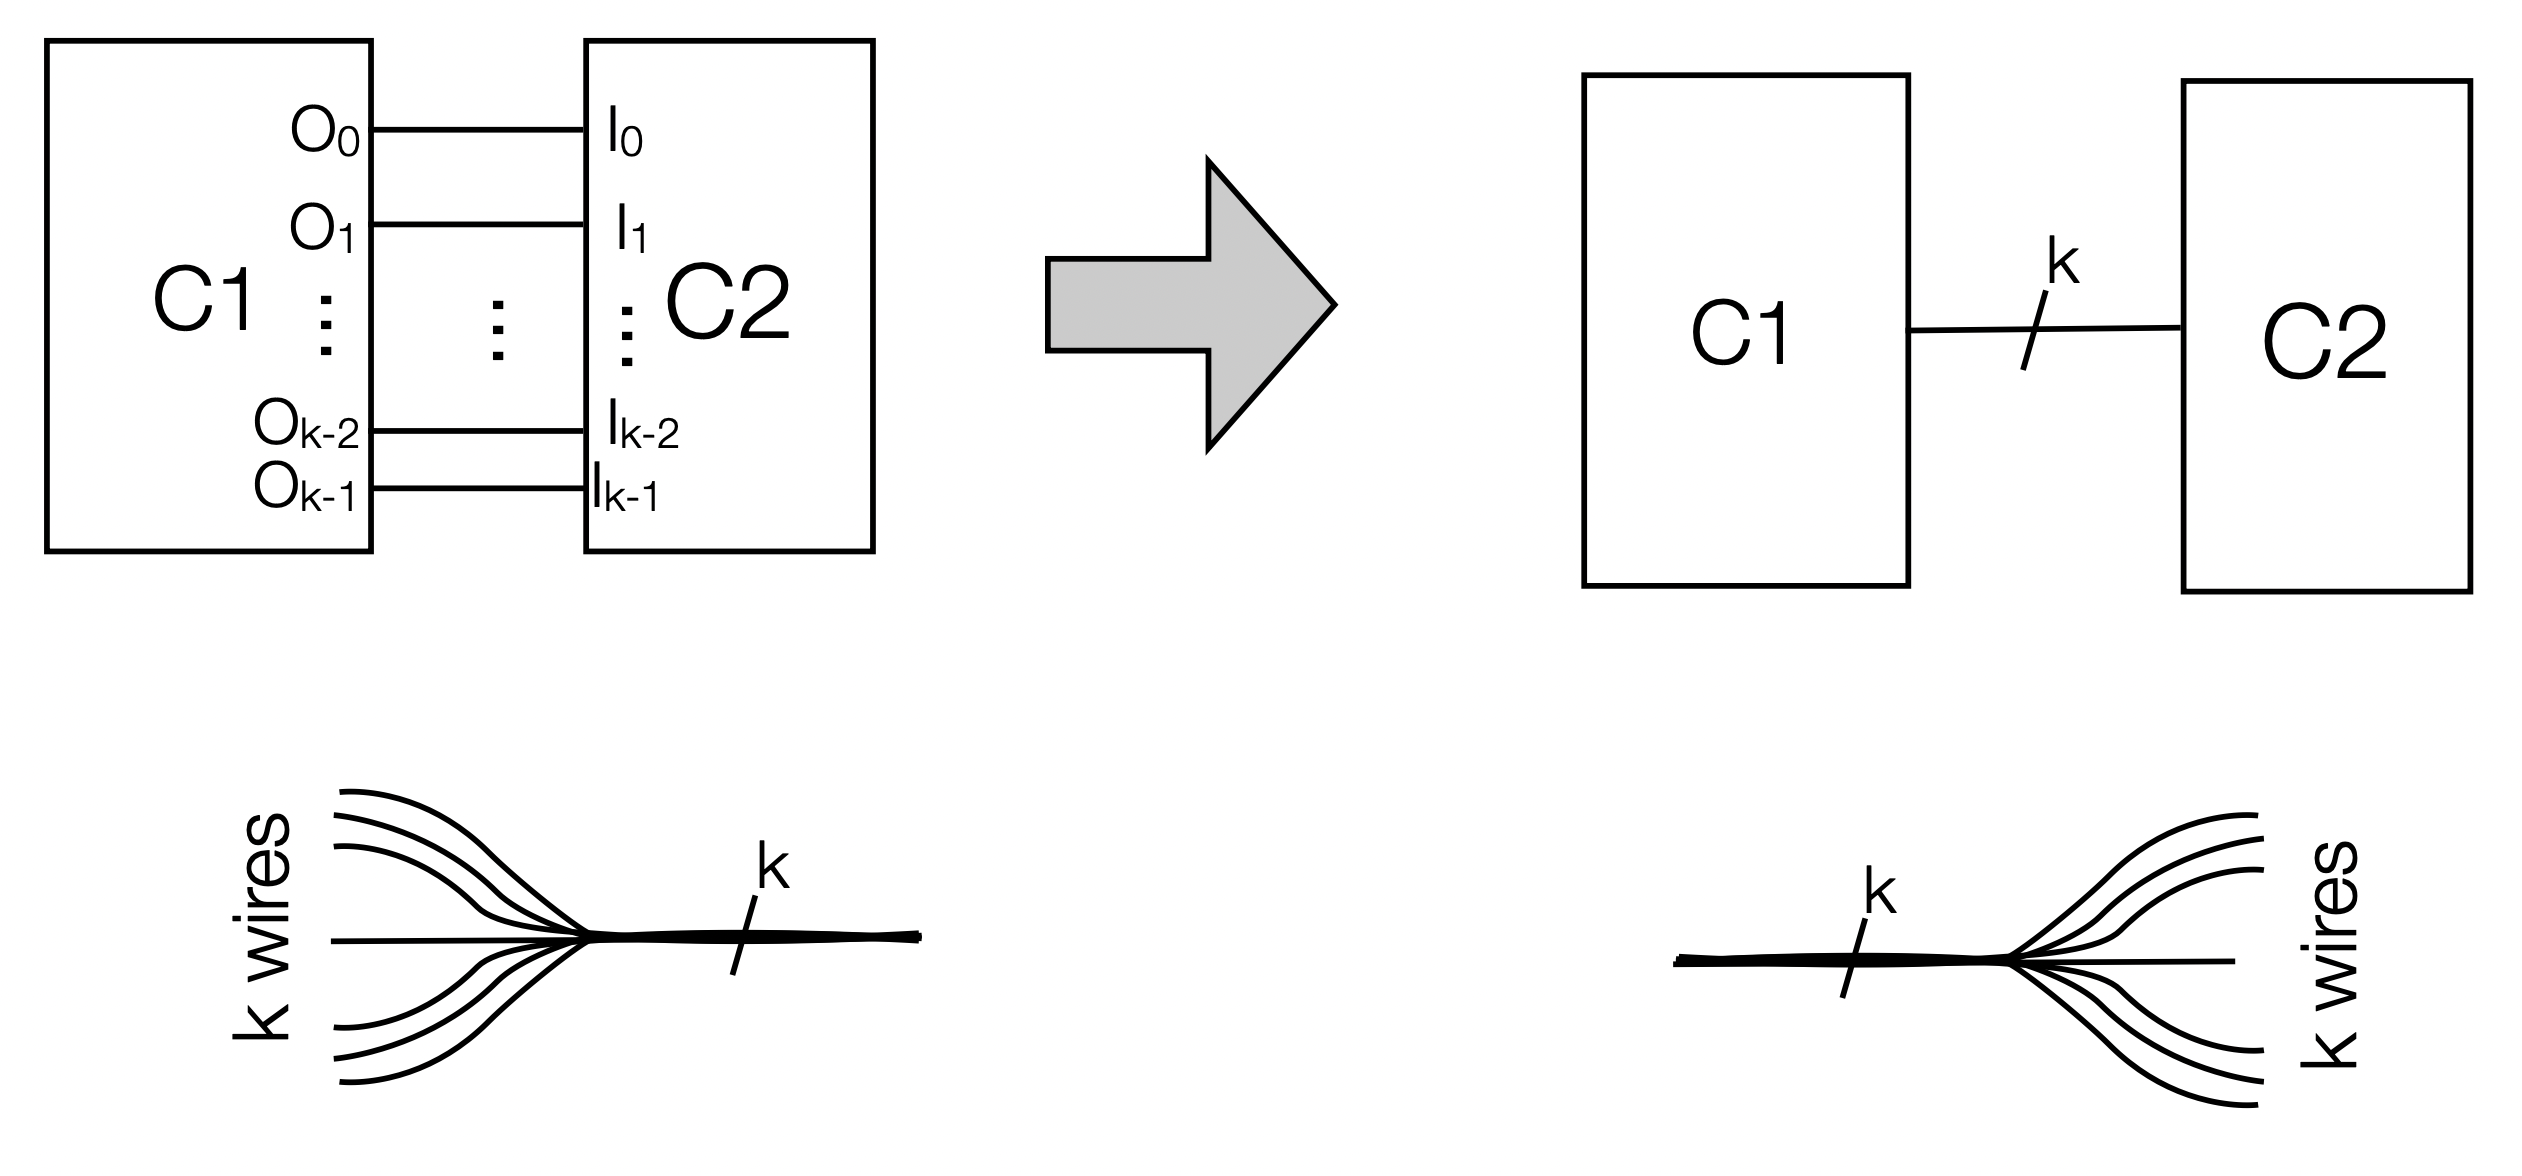
\includegraphics[width = 8cm]{img/multi.png}
        \end{figure}
        \item But remember: these are just wires
        \begin{itemize}
            \item E.g. how to get the MSB of a $k$-bit number represented by $k$ wires?
        \end{itemize}
    \end{itemize}
\end{frame}

\subsection{Combinational Circuits}
\begin{frame}{\secname: \subsecname}
    \begin{itemize}
        \item Enabler: for \enquote{turning on/off} inputs
        \begin{itemize}
            \item High-level circuit for other circuits, \enquote{enable} functionality can be added with an input labelled \enquote{E}
        \end{itemize}
        \item Decoder: set one of $2^k$ outputs to $1$ (others are $0$) based on unsigned binary representation of $k$-bit input
        \item Multiplexer (MUX): pass one of $2^k$ inputs as output based on $k$-bit \enquote{selector} input
        \item Shifter: shifts bits of $k$-bit input
        \begin{itemize}
            \item Can have input to control how much bits are shifted by, or can be hardcoded
        \end{itemize}
        \item Adders (unsigned, 2's complement): half/full adders can make ripple carry adder
        \begin{itemize}
            \item Carry lookahead also exists (reduced depth with increased parallelism)
        \end{itemize}
    \end{itemize}
\end{frame}

\subsection{Decoder/MUX Notation}
\begin{frame}{\secname: \subsecname}
    \begin{itemize}
        \item Must label everything in your combinational circuits
        \item Consider the two MUXes:
    \end{itemize}
    \begin{figure}[H]
        \centering
        \begin{tikzpicture}
            \tikzset{mux 4by2/.style={muxdemux, muxdemux def={Lh=4, NL=4, Rh=3, NB=1, w=2.5, square pins=1}}}
            \node [mux 4by2](muxbad) at (-5, 0) {MUX};
            \node [mux 4by2](mux) at (0, 0) {MUX};
            \node () at (-0.55, 0.84) {\tiny 0};
            \node () at (-0.55, 0.27) {\tiny 1};
            \node () at (-0.55, -0.27) {\tiny 2};
            \node () at (-0.55, -0.84) {\tiny 3};
            \node () at (0, -0.75) {\tiny S};
            \node () at (0, 0.75) {\tiny E};
        \end{tikzpicture}
    \end{figure}
\end{frame}

\section{Homework 2}
\subsection{Problem 1}
\begin{frame}{\secname: \subsecname}
    Simplify the following Boolean expressions to a minimum number of literals:
    \begin{enumerate}[(a)]
        \item $\overbar{B}C + \overbar{B}\overbar{C}D$
        \item $\overbar{(\overbar{Y} + Z)}(Y + \overbar{Z})$
        \item $\overbar{C}\overbar{D} + C\overbar{D}A + DA$
        \item $X(\overbar{C}Y + \overbar{C}\overbar{Y}) + X(\overbar{W}\overbar{C} + \overbar{W}C)$
        \item $(\overbar{B}\overbar{C} + BD + \overbar{C}D)(\overbar{B} + C + \overbar{B}C)$
    \end{enumerate}
\end{frame}

\subsection{Problem 2}
\begin{frame}{\secname: \subsecname}
    Reduce the following Boolean expressions to the indicated number of literals:
    \begin{enumerate}[(a)]
        \item $Y + \overbar{Z}(W + \overbar{Y + W})$ to two literals
        \item $\overbar{Y}X + Y\overbar{X}Z + \overbar{Y}\overbar{X}$ to three literals
        \item $\overbar{Y}X(\overbar{W} + ZW) + X(Y + \overbar{Y}\overbar{Z}W)$ to one literal
    \end{enumerate}
\end{frame}

\subsection{Problem 3}
\begin{frame}{\secname: \subsecname}
    Using DeMorgan’s theorem (as many times as necessary), express the function $F = \overbar{X}Z + X\overbar{Z}Y + \overbar{X}\overbar{Y}$ with only:
    \begin{enumerate}[(a)]
        \item OR and complement operations
        \item AND and complement operations
    \end{enumerate}
\end{frame}

\subsection{Problem 4}
\begin{frame}{\secname: \subsecname}
    Find the complement of the following expressions:
    \begin{enumerate}[(a)]
        \item $\overbar{B}\overbar{D} + BD$
        \item $(C + \overbar{B}D)(C + \overbar{B} + \overbar{D})(\overbar{C}\overbar{B} + \overbar{D})$
        \item $\overbar{W}\overbar{Y}(Z\overbar{X} + \overbar{Z}X) + WY(Z + X)(\overbar{Z} + \overbar{X})$
        \item $(\overbar{B} + \overbar{D})AC + E$
    \end{enumerate}
\end{frame}

\subsection{Problem 5}
\begin{frame}{\secname: \subsecname}
    Convert the following into sum-of-products and product-of-sums forms:
    \begin{enumerate}[(a)]
        \item $(\overbar{A} + \overbar{B}\overbar{D})(\overbar{D} + A\overbar{C})$
        \item $(\overbar{Z} + Y)\overbar{X}(\overbar{X} + Z) + X$
        \item $(\overbar{Z} + XW + \overbar{W}Y)(\overbar{X} + \overbar{Z}\overbar{Y})$
    \end{enumerate}
\end{frame}

\subsection{Problem 6}
\begin{frame}{\secname: \subsecname}
    Simplify the following boolean expressions using a K-map:
    \begin{enumerate}[(a)]
        \item $B\overbar{C} + CD + B\overbar{D} + \overbar{B}\overbar{C}D$
        \item $\overbar{Y}\overbar{Z} + \overbar{X}\overbar{Z} + ZX\overbar{Y}$
        \item $XW + \overbar{X}\overbar{Z} + X\overbar{Z}\overbar{W}$
    \end{enumerate}
\end{frame}

\subsection{Problem 7}
\begin{frame}{\secname: \subsecname}
    Simplify in Sum-of-product form via a K-map (indicate what you identify as prime implicants and essential prime implicants). Recall that $m(i)$ is the product term whose variables are complemented when and only when their position corresponds to a ’0’ in the binary representation of $i$, e.g., $m(5) = \overbar{W}X\overbar{Y}Z$.
    \begin{enumerate}[(a)]
        \item $F(W, X, Y, Z) = \sum m(0, 4, 5, 7, 9, 12, 13, 14)$
        \item $F(A, B, C, D) = \sum m(0, 1, 2, 4, 5, 8, 9, 10, 11, 13, 15)$
        \item $F(A, B, C, D) = \sum m(0, 2, 3, 5, 7, 8, 10, 11, 14, 15)$
        \item $F(W, X, Y, Z) = \sum m(0, 1, 2, 5, 6, 7, 8, 9, 10, 13, 14, 15)$
        \item $F(W, X, Y, Z) = \sum m(0, 1, 2, 5, 8, 9, 11, 12)$
        \item $F(A, B, C, D) = \sum m(1, 3, 6, 7, 9, 13, 14, 15)$
    \end{enumerate}
\end{frame}

\subsection{Problem 8}
\begin{frame}{\secname: \subsecname}
    Simplify into Sum-of-product form the following Boolean functions $F$ together with the don't care conditions $d$:
    \begin{enumerate}[(a)]
        \item $F(W, X, Y, Z) = \sum m(0, 1, 3, 5, 7), d(W, X, Y, Z) = \sum m(2, 4, 6)$
        \item $F(A, B, C, D) = \sum m(2, 6, 7, 11, 14, 15), d(A, B, C, D) = \sum m(0, 8, 12, 13)$
        \item $F(A, B, C, D) = \sum m(2, 7, 9, 10, 15), d(A, B, C, D) = \sum m(3, 6, 14)$
    \end{enumerate}
\end{frame}

\end{document}
